\documentclass{article}

% Language setting
% Replace `english' with e.g. `spanish' to change the document language
\usepackage[english]{babel}

% Set page size and margins
% Replace `letterpaper' with `a4paper' for UK/EU standard size
\usepackage[letterpaper,top=2cm,bottom=2cm,left=3cm,right=3cm,marginparwidth=1.75cm]{geometry}

% Useful packages
\usepackage{amsmath}
\usepackage{graphicx}
\usepackage[colorlinks=true, allcolors=blue]{hyperref}
\usepackage{float}
\usepackage{caption}
\usepackage{subfigure}

\title{lab01: Clustering Lab}
\author{Group 18}


\begin{document}
\maketitle

\section{SimpleKmeans}

\subsection{Choose a set of attributes for clustering and give a motivation.}

First we will work with the dataset “food” including nutrient levels of 27 kinds of food (see plot\ref{fig:data}).
At the beginning we implement SimpleKmeans on it with 2 clusters and attributes ”fat”, “protein” and “energy” . The motivation is that we can see from the dataset that there are meats and seafoods, which meats may have a higher fat and energy and seafood may have a higher protein, hope those attributes can help us classify them.  
\begin{figure}[H]
\centering
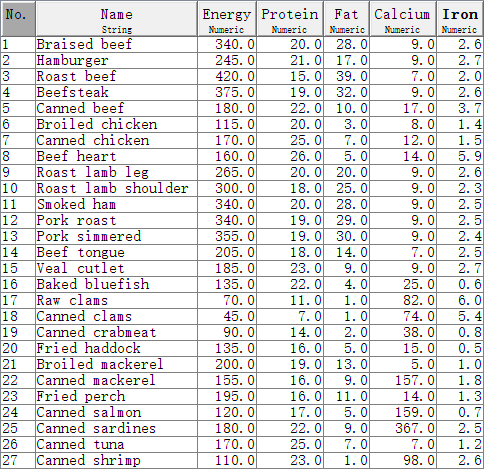
\includegraphics[width=0.7\textwidth]{data.png}
\caption{\label{fig:data}dataset:food}
\end{figure}

Attribute “name” is always ignored because it is merely a tag and don’t provide actual information to help us classify.

\subsection{Experiment with at least two different numbers of clusters, e.g. 2 and 5, but with the same seed value 10.(Hint: always ignore attribute "name". Why does the name attribute need to be ignored?)}
\subsubsection{2 clusters:}

\begin{figure}[H]
\centering
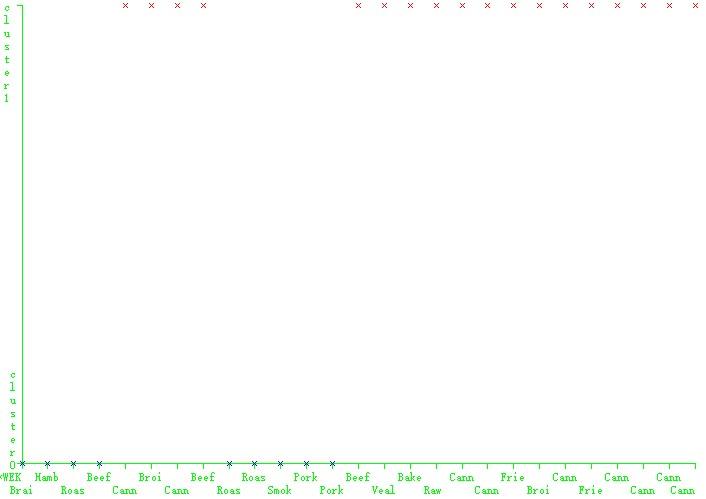
\includegraphics[width=0.8\textwidth]{k2EPF_cluster_p1.jpg}
\caption{\label{fig:k2EPF_cluster_p1}nametag vs cluster result}
\end{figure}


From the plot\ref{fig:k2EPF_cluster_p1} we can see that in general our goal is achieved but few kinds of meats with low fat\&energy are classified into another cluster which contains more seafoods, such as chicken, beef heart etc. And the protein doesn’t seems to work as we expected because most samples we have they have a similar protein level whether they are meat or fish(as we can see the low stddev of protein, see plot\ref{fig:protein} and \ref{fig:k2EPF_protain_p3}).

\begin{figure}[H]
\centering
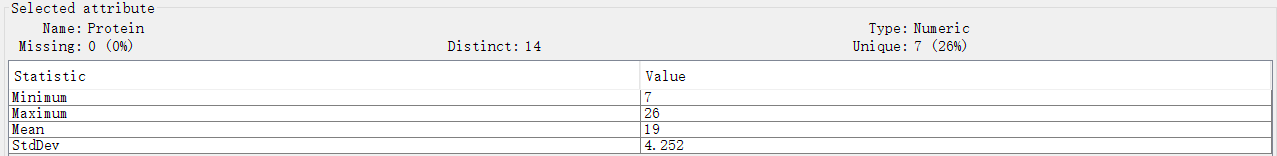
\includegraphics[width=1\textwidth]{attr_protein.png}
\caption{\label{fig:protein}attribute summary: protein}
\end{figure}
\begin{figure}[H]
\centering
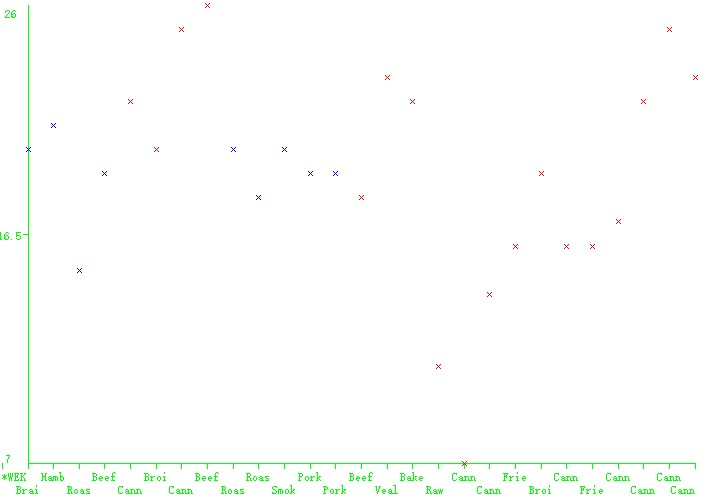
\includegraphics[width=0.8\textwidth]{k2EPF_protain_p3.jpg}
\caption{\label{fig:k2EPF_protain_p3}nametag vs protein}
\end{figure}

And from the energy-vs-fat plot\ref{fig:k2EPF_enrVSfat_p5} with plot\ref{fig:k2EPF_energy_p2} and \ref{fig:k2EPF_fat_p4} we can see that this 2 attributes are highly correlated so maybe we can consider that only keep 1 attribute of them as a choice 

\begin{figure}[H]
    \begin{minipage}[t]{0.5\linewidth}
        \centering
        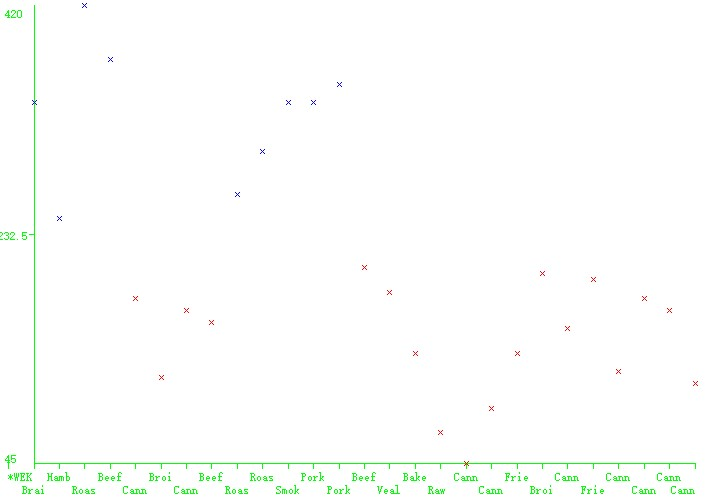
\includegraphics[scale = 0.4]{k2EPF_energy_p2.jpg}
        \caption{nametag vs energy}
        \label{fig:k2EPF_energy_p2}
    \end{minipage}
    \begin{minipage}[t]{0.5\linewidth}
        \centering
        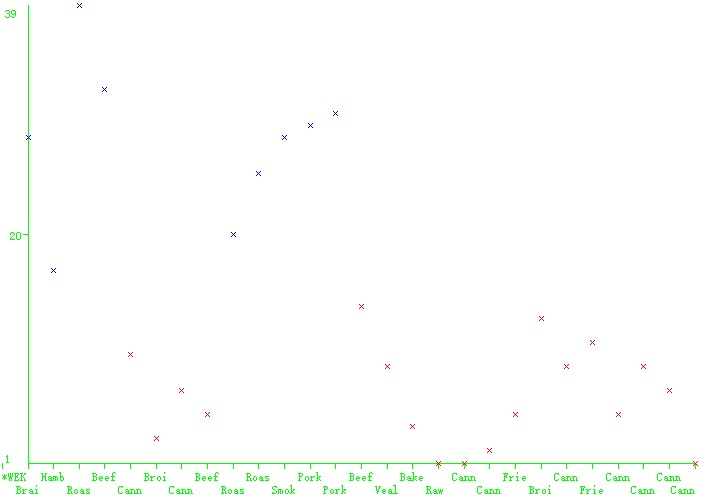
\includegraphics[scale = 0.4]{k2EPF_fat_p4.jpg}
        \caption{nametag vs fat}
        \label{fig:k2EPF_fat_p4}
    \end{minipage}
\end{figure}

\begin{figure}[H]
\centering
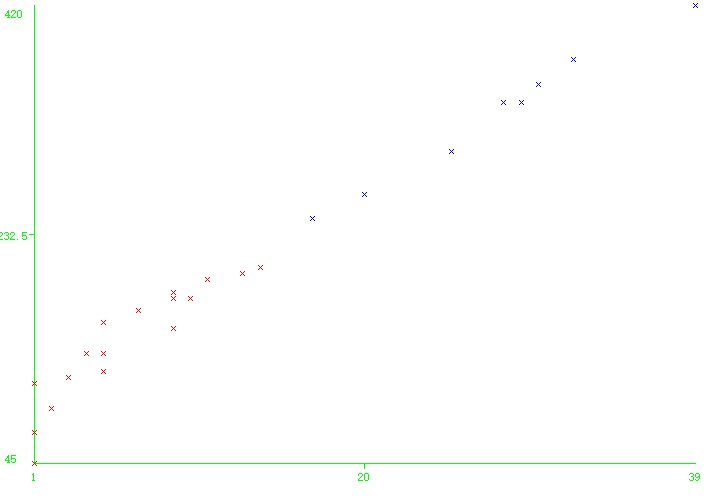
\includegraphics[width=0.8\textwidth]{k2EPF_enrVSfat_p5.jpg}
\caption{\label{fig:k2EPF_enrVSfat_p5}fat vs energy}
\end{figure}

\subsubsection{5 clusters:}
Now we try using cluster = 5 instead of 2:

\begin{figure}[H]
\centering
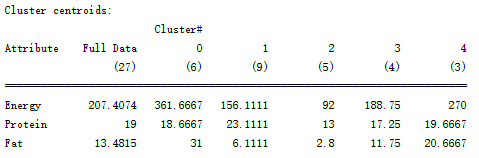
\includegraphics[width=0.8\textwidth]{k5s10_centroid.png}
\caption{\label{fig:k5s10_centroid} centroids of 5 clusters}
\end{figure}
From the results\ref{fig:k5s10_centroid} we can see that cluster 1 and 3 have similar centroid values which indicates that it might be better to merge them together.

\begin{figure}[H]
\centering
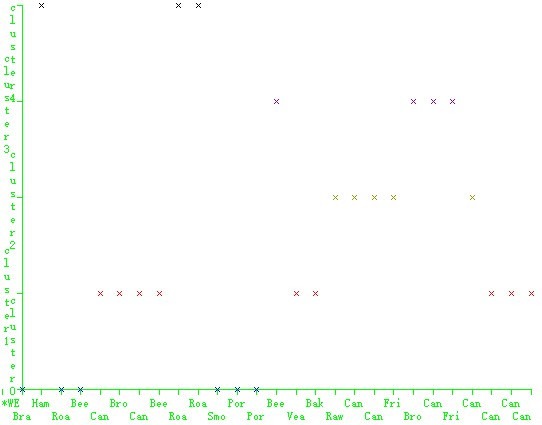
\includegraphics[width=0.8\textwidth]{k5EPF_cluster_p1.jpg}
\caption{\label{fig:k5EPF_cluster_p1} nametag vs cluster result under 5 clusters}
\end{figure}
From the plot we can see that there isn’t much useful information explicitly shown. Seems only 3 attributes we chose don’t works well for clustering into 5 clusters, for the reason that 2 attributes(fat and energy) are correlated and the other 1 attribute(protein) don’t have significant differences in general. So it may yield a similar result as using only fat to divide 5 clusters.

\subsection{Then try with a different seed value, i.e. different initial cluster centers. Compare the results with the previous results. Explain what the seed value controls.}
\begin{figure}[H]
\centering
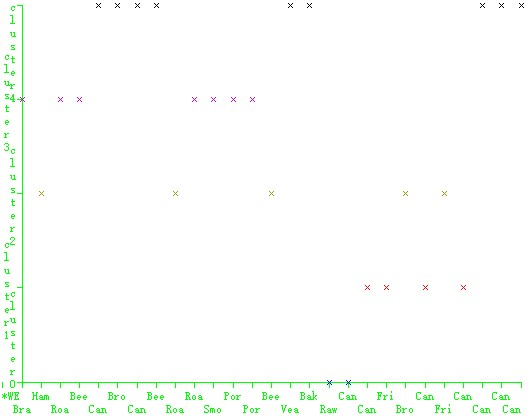
\includegraphics[width=0.8\textwidth]{k5EPF_seed2_cluster_p1.jpg}
\caption{\label{fig:k5EPF_seed2_cluster_p1} nametag vs cluster result under 5 clusters with seed 20}
\end{figure}

Now we try the same setting as cluster = 5 but set a different seed 20 instead of 10. Now we can see from the plotthat the result is completely different. The seed value control the randomness of the initial points choosing. Under kmeans we are using(with this dataset and attributes we chose) ,the initial points influences a lot when we have 5 clusters to divide into and obviously there isn't any same minimum which can easily be find by the algorithm. This can be reasoned by the conjecture we made, which is that out three attributes may not be able to provide more information than choosing solely 1 attribute energy/fat for classification so the lack of information provided brings the failure of effective clustering.

\subsection{Do you think the clusters are "good" clusters? (Are all of its members "similar" to each other? Are members from different clusters dissimilar?)}

As discussed above ,clustering 2 clusters is relatively good because it generally divided data points into meat and seafoods as what we expected. But clusters = 5 doesn.t seems to be good and heavily susceptible to the changing of initial points which makes the clustering result highly randomly, both the result with different seed don't have much similarity within clusters.

\subsection{What does each cluster represent? Choose one of the results. Make up labels (words or phrases in English) which characterize each cluster.}

In out first attempt with 2 clusters preset. We can label 1 as meats and another as seafoods nonetheless we have a considerable misclassification rate in label “seafoods”

\section{MakeDensityBasedClusters}

\subsection{Use the SimpleKMeans clusterer which gave the result you haven chosen in 5).}

We implement MakeDensityBasedClusters with mindev = 1e-6 based on SimpleKMeans clusster = 2(the first clustering in this report).

The clustering result is shown by the plot\ref{fig:MDk2EPF_mdev1e-6_cluster_p1}, and we can see that it's exactly the same with SimpleKMeans without MakeDensityBasedClusters, the clustering result hasn'e been changed at all.
\begin{figure}[H]
\centering
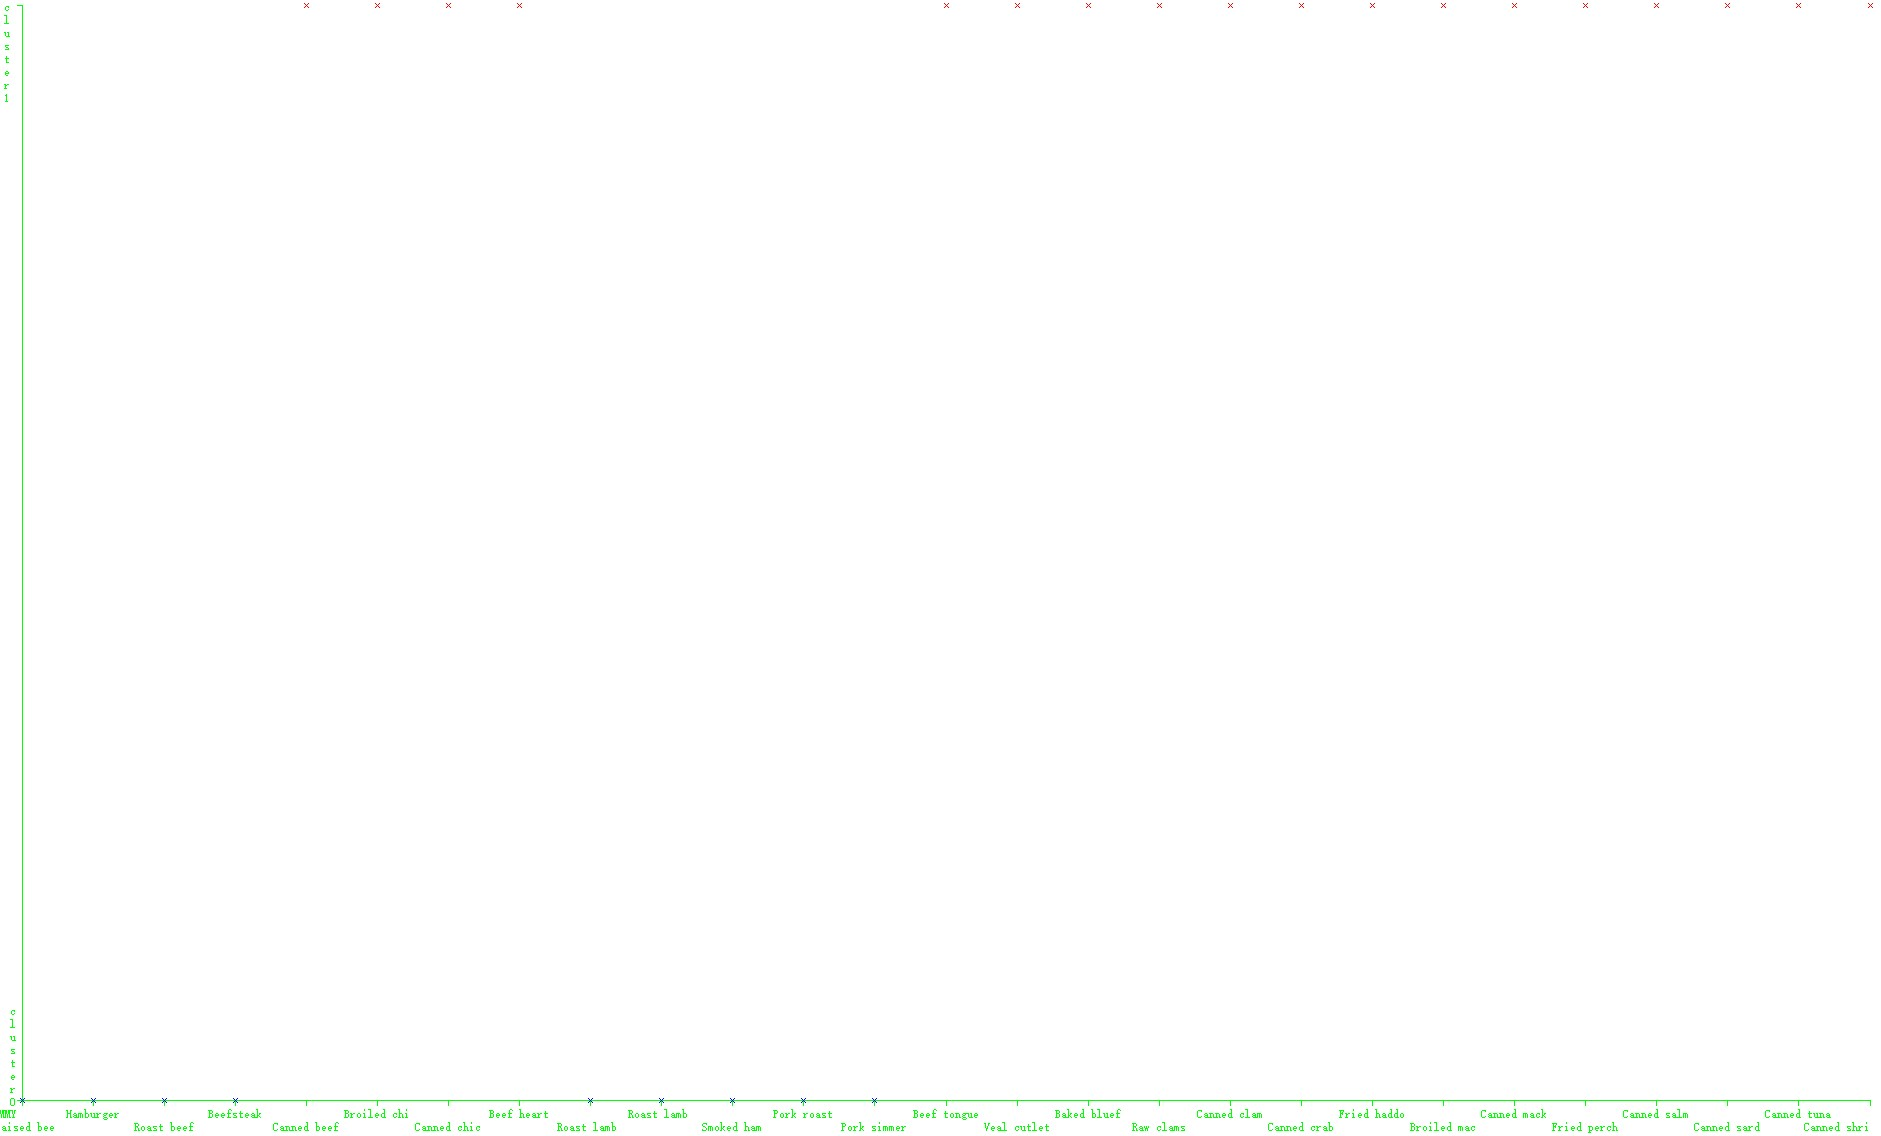
\includegraphics[width=0.8\textwidth]{MDk2EPF_mdev1e-6_cluster_p1.jpg}
\caption{\label{fig:MDk2EPF_mdev1e-6_cluster_p1} name vs cluster, mindev = 1e-6}
\end{figure}

\subsection{Experiment with at least two different standard deviations. Compare the results. (Hint: Increasing the standard deviation to higher values will make the differences in different runs more obvious and thus it will be easier to conclude what the parameter does)}

\begin{figure}[H]
\centering
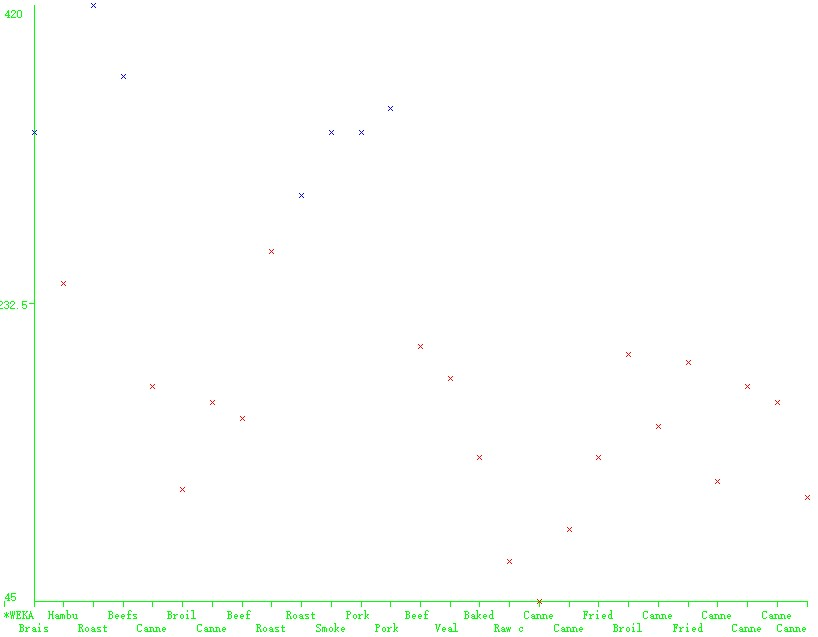
\includegraphics[width=0.8\textwidth]{MDk2EPF_mdev100_cluster_p1.jpg}
\caption{\label{fig:MDk2EPF_mdev100_cluster_p1} name vs cluster, mindev = 100}
\end{figure}
\begin{figure}[H]
\centering
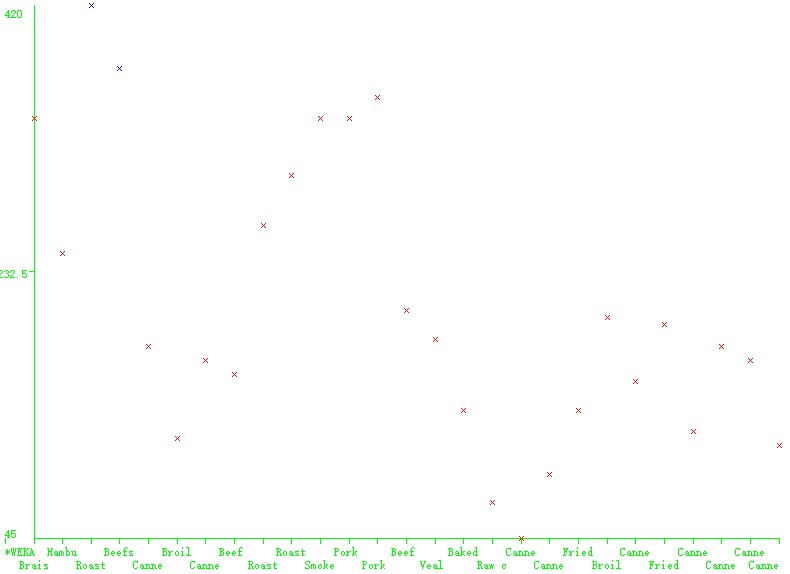
\includegraphics[width=0.8\textwidth]{MDk2EPF_mdev200_cluster_p1.jpg}
\caption{\label{fig:MDk2EPF_mdev200_cluster_p1} name vs cluster, mindev = 200}
\end{figure}

When we set mindev as 100(p\ref{fig:MDk2EPF_mdev100_cluster_p1}) and 200(p\ref{fig:MDk2EPF_mdev200_cluster_p1}) we can see that 1 of the cluster is became more and more comprehensive when mindev rises. Which we can conjecture that the large mindev value allow the cluster have larger range and finally 1 cluster will devour  all of the data points if we set the mindev even higher.

\end{document}